Como explicado por \citeonline{Camargo2022}, \gls{lora} é uma tecnologia, patenteada e desenvolvida pela Semtech, que tem como foco viabilizar a transmissão de dados sem fio em longo alcance através de radiofrequência.

A rede \gls{lorawan} é constituída por dispositivos finais, gateways e servidores de rede/aplicação.
Com o objetivo de realizar um gerenciamento mais fino de consumo energético, a comunicação entre os dispositivos finais e servidores de rede são definidos por três classes como demonstrado na tabela~\ref{tab:tabela_classes}.

\begin{table}[H]
    \centering
    \caption{Classes de Configuração LoRa}
    \label{tab:tabela_classes}
    \begin{tabular}{|l|p{6cm}|p{6cm}|}
        \toprule
        \textbf{Classe} & \textbf{Descrição} & \textbf{Característica} \\
        \midrule
        Classe A & O dispositivo final é habilitado à receber downlink imediatamente após ser realizado um envio de mensagem (uplink). & Menor consumo energético e menor tráfego de mensagens. \\
        \midrule
        Classe B & O dispositivo final é habilitado à receber downlink em períodos agendados e conhecidos. & Consumo energético significantemente maior que a classe A, mas viabiliza comunicação mais frequente entre servidor e dispositivo final. \\
        \midrule
        Classe C & O dispositivo final é continuamente habilitado à receber downlink. & Consumo energético muito alto, mas viabiliza a comunicação entre as partes de forma quase ininterrupta.  \\
        \bottomrule
    \end{tabular}
    \begin{quote}
        Fonte: Adaptado de Semtech Corporation \cite{semtech2024an1200_87}.
    \end{quote}
\end{table}

\begin{figure}[H]
    \centering
    \caption{Campos contidos em um pacote de Uplink}
    \label{fig:lora_uplink}
    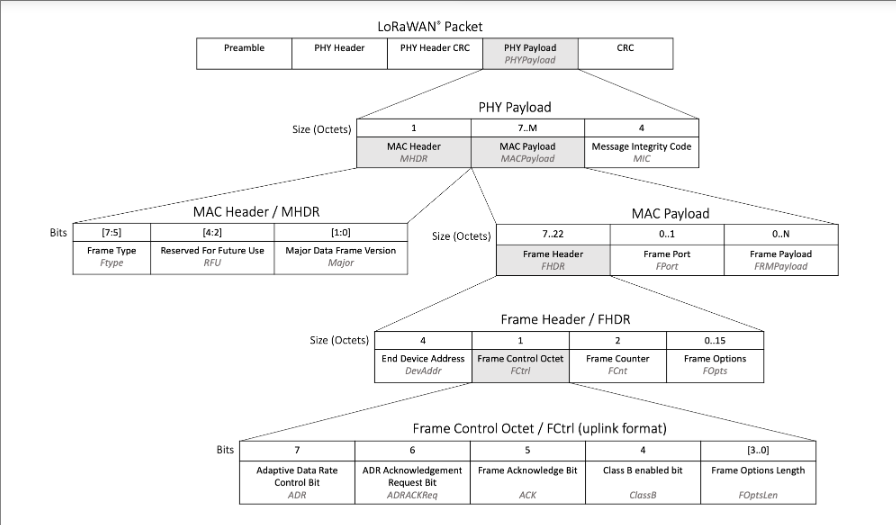
\includegraphics[width=0.85\textwidth]{sections/imagens/SemTech_Uplink_Dataframe.png}
    \small
    \begin{quote}
        Fonte: Adaptado de Semtech Corporation \cite{semtech2024an1200}.
    \end{quote}
\end{figure}

A figura~\ref{fig:lora_uplink} apresenta a estrutura de pacote de rede que é utilizado na tecnologia LoRa. 
Tal estrutura é utilizada tanto no envio de dados pelo dispositivo final (uplink), quanto no recebimento de dados (downlink).

\begin{figure}[H]
    \centering
    \caption{Campos contidos em Frame Header em Downlink}
    \label{fig:fhdr_lora_downlink}
    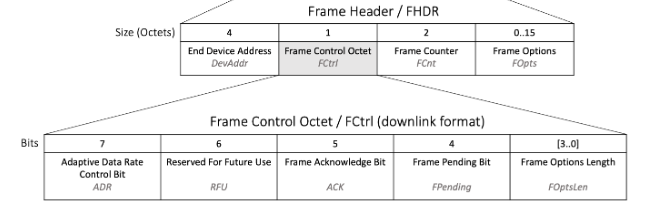
\includegraphics[width=0.85\textwidth]{sections/imagens/SemTech_Downlink_Dataframe.png}
    \small
    \begin{quote}
        Fonte: Adaptado de Semtech Corporation \cite{semtech2024an1200}.
    \end{quote}
\end{figure}

A estrutura do pacote de rede de uplink e downlink é a mesma, mas há diferenças em flags específicas entre os tipos de transmissão de dados. 
A figura~\ref{fig:fhdr_lora_downlink} apresenta a estrutura do “Frame Header / FHDR“ utilizada em downlink, as estruturas de pacote divergiam-se na flag de classe B, para uplink, onde o dispositivo final informa ao servidor estar no modo de recebimento de mensagens em tempo programado, e no pacote downlink, há a flag de FPeding, onde tal flag é utilizada para informar a existência de mais mensagens à serem enviadas pelo servidor/getaway.

Conforme apresentado pela \citeonline{lora_alliance_rp002_105} o tamanho máximo de MACPayload, respeitando o padrão regulatório AU915, que será melhor explicado e abordado posteriormente, em bytes é variável e dependente do tamanho ocupado pelo atributo Fopts, que é utilizado para solicitar alterações de parâmetros de rede ao dispositivo final.
Não utilizando repetidores de sinal que interligam dispositivos finais com gateways, o tamanho máximo de MACPayload é de 250 bytes, restando em torno de 227 bytes utilizáveis em \gls{payload}.

Para viabilizar a modulação LoRa em dispositivo final, é necessário realizar a configuração de três fundamentais parâmetros. 
A tabela~\ref{tab:parametros_lora} apresenta as definições dos principais parâmetros que ajustam o funcionamento da rede \gls{lorawan}.

\begin{table}[H]
    \centering
    \caption{Parâmetros de Configuração LoRa}
    \label{tab:parametros_lora}
    \begin{tabular}{|l|p{6cm}|}
        \toprule
        \textbf{Parâmetro} & \textbf{Definição} \\
        \midrule
        
        \gls{bw} & Determina a capacidade máxima de transmissão em determinado período de tempo (medido em kHz).\\
        \midrule
        
        \gls{sf} & Determina o alcânce de sinal de rádio, o SF é determinado por classes onde quanto maior a classe maior a área de alcance do sinal.\\
        \midrule
        
        \gls{cr} & Número de Bits destinado à redundância de dados, utilizado para possibilitar recuperação da mensagem em caso de erros na transmissão.\\
        \bottomrule
    \end{tabular}
    \begin{quote}
        Fonte: Adaptado de \citeonline{Camargo2022}.
    \end{quote}
\end{table}